\documentclass{standalone}
\usepackage{tikz}
\usepackage{ctex,siunitx}
\usepackage{tkz-euclide}
\usepackage{amsmath}
\usetikzlibrary{patterns, calc}
\usetikzlibrary {decorations.pathmorphing, decorations.pathreplacing, decorations.shapes,}
\begin{document}
\small
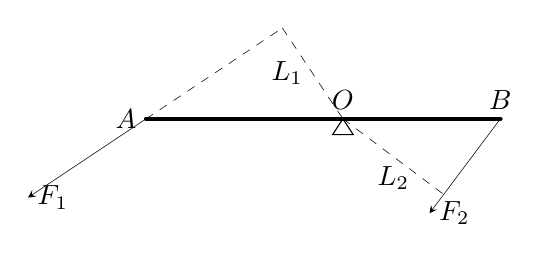
\begin{tikzpicture}[>=stealth]
  \tkzDefPoints{-2.5/0/A, 2/0/B, 0/0/O, -4/-1/F_1, 1.1/-1.2/F_2}
  \tkzDrawSegments[ultra thick](A,B)
  \tkzDrawSegments[->](A,F_1 B,F_2)
  \tkzLabelPoints[above](O,B)
  \tkzLabelPoints[left](A)
  \tkzLabelPoints[right](F_1,F_2)
  \tkzDefPointBy[projection= onto A--F_1](O)\tkzGetPoint{A'}
  \tkzDefPointBy[projection= onto B--F_2](O)\tkzGetPoint{B'}
  \tkzDrawSegments[dashed](A,A' A',O O,B')
  \tkzLabelSegment[left](O,A'){$L_1$}
  \tkzLabelSegment[below](O,B'){$L_2$}
  \draw(O)--(-.13,-.2)--(.13,-.2)--(O);
\end{tikzpicture}
\end{document}